\begin{figure}[htbp]
\centering
\makebox[\textwidth][c]{%
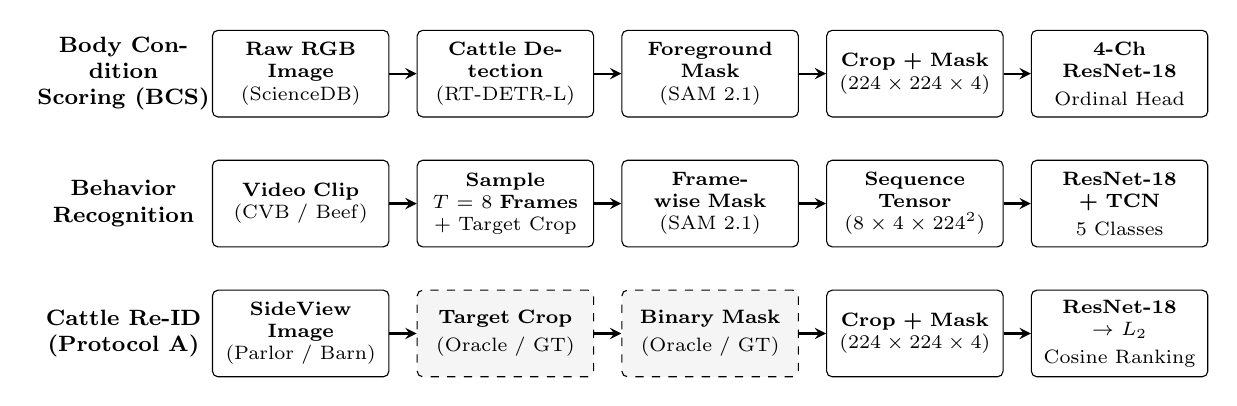
\begin{tikzpicture}[
  tag/.style={font=\bfseries\footnotesize, align=center, text width=2.2cm},
  box/.style={draw, rectangle, rounded corners=2pt, align=center, font=\scriptsize, minimum height=1.1cm, text width=2.1cm, fill=white, inner sep=2pt},
  oraclebox/.style={draw, rectangle, rounded corners=2pt, dashed, align=center, font=\scriptsize, minimum height=1.1cm, text width=2.1cm, fill=gray!8, inner sep=2pt},
  arrow/.style={->, >=stealth, thick}
]

% Row 1: BCS Pipeline
\node[tag] (t1) at (1.1, 0.0) {Body Condition\\Scoring (BCS)};
\node[box] (bcs1) at (3.35, 0.0) {\textbf{Raw RGB Image}\\(ScienceDB)};
\node[box] (bcs2) at (5.95, 0.0) {\textbf{Cattle Detection}\\(RT-DETR-L)};
\node[box] (bcs3) at (8.55, 0.0) {\textbf{Foreground Mask}\\(SAM 2.1)};
\node[box] (bcs4) at (11.15, 0.0) {\textbf{Crop + Mask}\\($224\times224\times4$)};
\node[box] (bcs5) at (13.75, 0.0) {\textbf{4-Ch ResNet-18}\\[2pt]Ordinal Head};

\draw[arrow] (bcs1) -- (bcs2);
\draw[arrow] (bcs2) -- (bcs3);
\draw[arrow] (bcs3) -- (bcs4);
\draw[arrow] (bcs4) -- (bcs5);

% Row 2: Behavior Pipeline
\node[tag] (t2) at (1.1, -1.65) {Behavior\\Recognition};
\node[box] (beh1) at (3.35, -1.65) {\textbf{Video Clip}\\(CVB / Beef)};
\node[box] (beh2) at (5.95, -1.65) {\textbf{Sample $T=8$ Frames}\\+ Target Crop};
\node[box] (beh3) at (8.55, -1.65) {\textbf{Frame-wise Mask}\\(SAM 2.1)};
\node[box] (beh4) at (11.15, -1.65) {\textbf{Sequence Tensor}\\($8\times4\times224^2$)};
\node[box] (beh5) at (13.75, -1.65) {\textbf{ResNet-18 + TCN}\\[2pt]5 Classes};

\draw[arrow] (beh1) -- (beh2);
\draw[arrow] (beh2) -- (beh3);
\draw[arrow] (beh3) -- (beh4);
\draw[arrow] (beh4) -- (beh5);

% Row 3: Re-ID Pipeline
\node[tag] (t3) at (1.1, -3.3) {Cattle Re-ID\\(Protocol A)};
\node[box] (reid1) at (3.35, -3.3) {\textbf{SideView Image}\\(Parlor / Barn)};
\node[oraclebox] (reid2) at (5.95, -3.3) {\textbf{Target Crop}\\[2pt](Oracle / GT)};
\node[oraclebox] (reid3) at (8.55, -3.3) {\textbf{Binary Mask}\\[2pt](Oracle / GT)};
\node[box] (reid4) at (11.15, -3.3) {\textbf{Crop + Mask}\\($224\times224\times4$)};
\node[box] (reid5) at (13.75, -3.3) {\mbox{\textbf{ResNet-18}} $\to$ $L_2$\\[2pt]Cosine Ranking};

\draw[arrow] (reid1) -- (reid2);
\draw[arrow] (reid2) -- (reid3);
\draw[arrow] (reid3) -- (reid4);
\draw[arrow] (reid4) -- (reid5);

\end{tikzpicture}%
}
\caption[Task-specific cattle-centered input pipelines]{Task-specific cattle-centered input pipelines for body condition scoring, behavior recognition, and individual re-identification. In BCS and behavior recognition, target cow localization and foreground segmentation are generated automatically via RT-DETR-L and SAM 2.1. In cattle re-identification, target bounding boxes and binary masks are obtained from released ground-truth annotations (oracle setting, dashed boxes), strictly avoiding automatic perception errors during cross-setting retrieval evaluation.}
\label{fig:task_representation_pipeline}
\end{figure}
